% settings for the plots in this chapter
\def \myplotswitdth {0.95}

\chapter{Results}
\label{chapter:results}
Our simulator allows to test the Bitcoin protocol under different conditions:
it is possible to choose the size of the network and the delay of messages between nodes.
It is also easy to simulate network attacks by simply changing the transport layer used or by adding a new layer on top of the default one.

\medskip
This chapter covers our experiments with Bitcoin.
First, we analyze the protocol at rest to obtain a baseline of its performances;
then, we introduce delays on the communications between nodes to check if a degraded network infrastructure affects the protocol;
finally we simulate different variants of the Balance attack (\cref{sec:balance}) and compare their effects on Bitcoin.


\section{Settings}
We run each simulation multiple times with different seeds for the random number generators to obtain higher statistical significance for the results.
Each run simulates \num{3} hours of activity of the Bitcoin protocol.
The parameter that regulates the blocks creation rate of the miners is tuned so that a new block is generated on average every \num{10} minutes.
Since we do not simulate attacks that completely isolate nodes from each other or interfere with the control messages, we have disabled the ping-pong mechanism used by Bitcoin to verify that TCP connections are still alive:
this allowed us to spare computational resources and run the same simulation multiple times with more different seeds.


\section{Parameters}
The simulator accepts different parameters that allow to change the settings of the simulation.
All parameters can be changed independently of each other and are specified in the configuration file.
In particular, the simulator accepts the following \num{5} values:
\begin{enumerate}
	\item \texttt{network\_size};
	\item \texttt{delay};
	\item \texttt{balance\_attack\_delay};
	\item \texttt{balance\_attack\_drop};
	\item \texttt{balance\_attack\_partitions}.
\end{enumerate}

\paragraph{Network Size}
The \texttt{network\_size} parameter controls the number of nodes simulated.
It can vary from \num{1} to a potentially unlimited number, which is only bounded by the available computational resources.
Since the Bitcoin network has about \num{9000} active node on average at the time of writing, we run simulations up to \num{10000} nodes.

\paragraph{Delay}
The \texttt{delay} parameter controls the average delay of messages exchanged between Bitcoin nodes.
The delay of each message is randomly chosen from a uniform distribution in $[-\texttt{delay}, +\texttt{delay}]$.

\paragraph{Balance Attack Delay}
The \texttt{balance\_attack\_delay} parameter controls the magnitude of the simulated Balance attack:
it adds an additional delay to all messages of type \texttt{Block} exchanged by nodes belonging to different partitions.
The delay is added to the base network delay controlled by the \texttt{delay} parameter.

\paragraph{Balance Attack Drop}
The \texttt{balance\_attack\_drop} parameter controls the drop rate of \texttt{Block} messages exchanged by nodes belonging to different partitions.
Please note that this is an extension to the Balance attack described in \cite{balance_attack_2017}, since the paper does not consider dropping messages between nodes.

\paragraph{Balance Attack Partitions}
The \texttt{balance\_attack\_partitions} parameter controls the number of partitions of equal size in which the nodes of the network are divided by the Balance attack.
The setting discussed in the original paper is to partition the network in two parts only.


\section{Experiments}
Most attacks against Bitcoin aim at double spending the money.
Forks on the blockchain allow an attacker to easily achieve double spending attacks.
The main metric used to evaluate the performances of the protocol is thus the number of forks in the blockchain.
Forks happen with a non-zero probability even at rest in Bitcoin due to some inevitable delays on the information propagation;
degraded network conditions and a wide range of attacks can increase the probability of forks and open the possibility for double-spend attempts.

\subsection{Protocol at rest}
We run the simulations for different network sizes and $\texttt{delay} = \SI{50}{\milli\second}$, similar to the delay of a normal TCP connection over the Internet.
Under these conditions, the Bitcoin nodes exchange $8$ \texttt{Version}, \texttt{VerAck}, \texttt{GetAddr} and \texttt{Addr} messages each:
each node connects to exactly \num{8} peers and each connection generates a single exchange of the above control messages.

\begin{figure}[h!]
	\centering
	% \vspace*{0.25}
	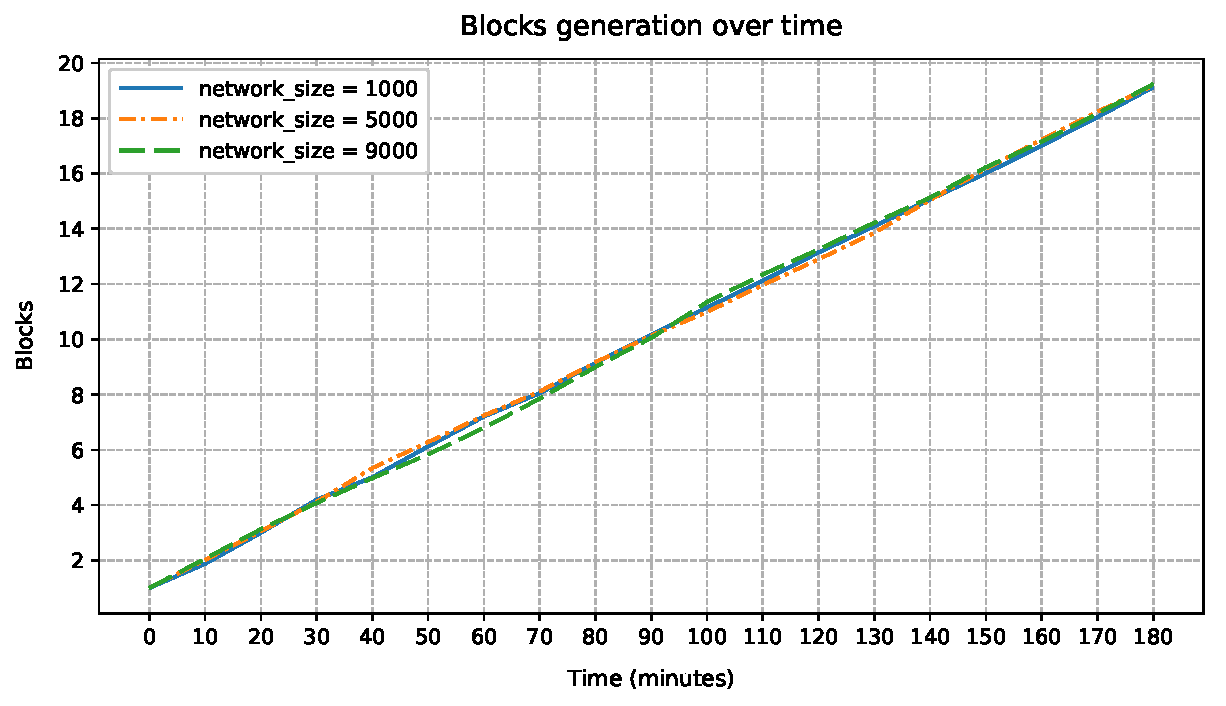
\includegraphics[width=\myplotswitdth \columnwidth]{plots/blocks_rest_linechart}
	\caption[Blocks generation for networks of different sizes]{
		Blocks generation for networks of different sizes under normal conditions:
		\SI{50}{\milli\second} delay on average and no attack in progress.
		At time \num{0}, only the genesis block is present.
		During the simulation, a new block is generated on average every \num{10} minutes, regardless of the network's size.
	}
	\label{fig:blocks-rest-linechart}
\end{figure}

\cref{fig:blocks-rest-linechart} shows that the network generated on average \num{18} blocks during the simulation of \num{3} hours (\num{1} block every \num{10} minutes), independently on the size of the network.
The plot shows the results for networks of \num{1000}, \num{5000} and \num{9000} nodes, but the same behavior is valid for all sizes in between.
Under these conditions, the Bitcoin protocol does not produce any fork in our simulations.

\subsection{Generalized network delays}
We run experiments for different network sizes and incremental delays from \num{0} to \SI{30}{\second} with steps of \SI{5}{\second} in the propagation of each message.
Generalized network delays on the network does not influence the number of control messages exchanged.
Similar to the previous experiment, the network generates \num{1} block every \num{10} minutes on average.

\medskip
\cref{fig:forks-delay-1000} shows the number of forks generated a the network of \num{1000} nodes over time and their distribution at the end of the simulation.
The effect of network delays is a general increase in the number of forks:
with a delay of \SI{0}{\second}, the network never generates forks;
small delays of \num{5} or \SI{10}{\second} already cause the generation of \num{1} to \num{3} forks in some simulations;
longer delays of \num{15} to \SI{30}{\second} produce forks in a significantly higher number of simulations.

\begin{figure}[ht]
	\begin{subfigure}{\textwidth}
		\centering
		% \vspace*{0.25cm}
		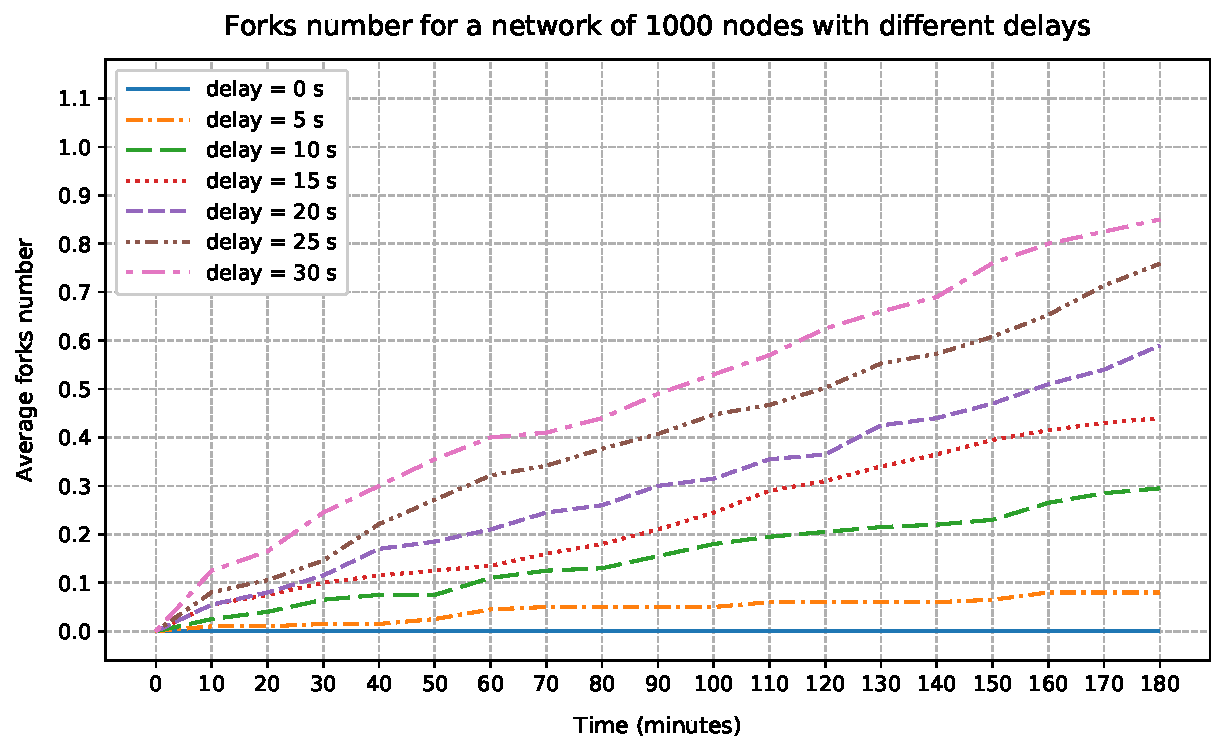
\includegraphics[width=\myplotswitdth \columnwidth]{plots/forks_delay_1000_linechart}
		\vspace*{0.25cm}
		\caption{
			Average forks number for a network of \num{1000} nodes with different delays.
			In perfect conditions of zero delay, Bitcoin nodes never generate forks.
			Longer delays cause a faster increasing number of forks over time.
		}
		\vspace*{0.75cm}
	\end{subfigure}
	\begin{subfigure}{\textwidth}
		\centering
		\vspace*{0.25cm}
		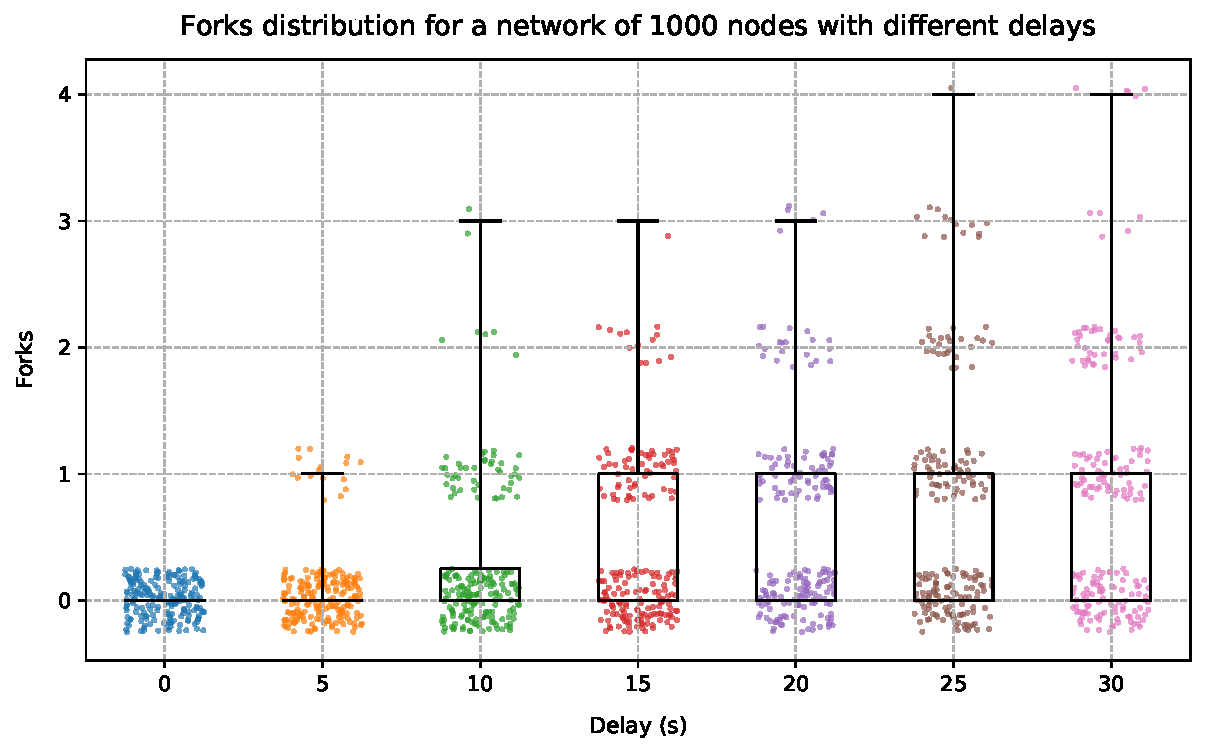
\includegraphics[width=\myplotswitdth \columnwidth]{plots/forks_delay_1000_boxplot}
		\vspace*{0.25cm}
		\caption{
			Distribution of forks for a network of \num{1000} nodes with different delays.
			With zero delay, blocks are immediately distributed to all nodes and no fork is generated.
			Even with a small delay of \SI{5}{\second}, the network starts to create some forks.
			Longer delays produce an higher number of forks.
		}
		\vspace*{0.25cm}
	\end{subfigure}
	\caption[Forks distribution for a network of 1000 nodes with different delays]{
		Forks distribution for a network of \num{1000} nodes with different delays.
	}
	\label{fig:forks-delay-1000}
\end{figure}

\medskip
Similar results yield for bigger networks.
\cref{fig:forks-delay-9000} show the effect of delays on the forks generated by a network of \num{9000} nodes:
the number of forks seems to be linearly correlated with the message's delay.
The effect of the delays seems to be also related to the size of the network:
the network with \num{9000} nodes produces on average \num{0.1} to \num{0.2} forks more that the one with \num{1000} nodes for each tested value of \texttt{delay} at the of the simulation.

\begin{figure}[ht]
	\begin{subfigure}{\textwidth}
		\centering
		% \vspace*{0.25cm}
		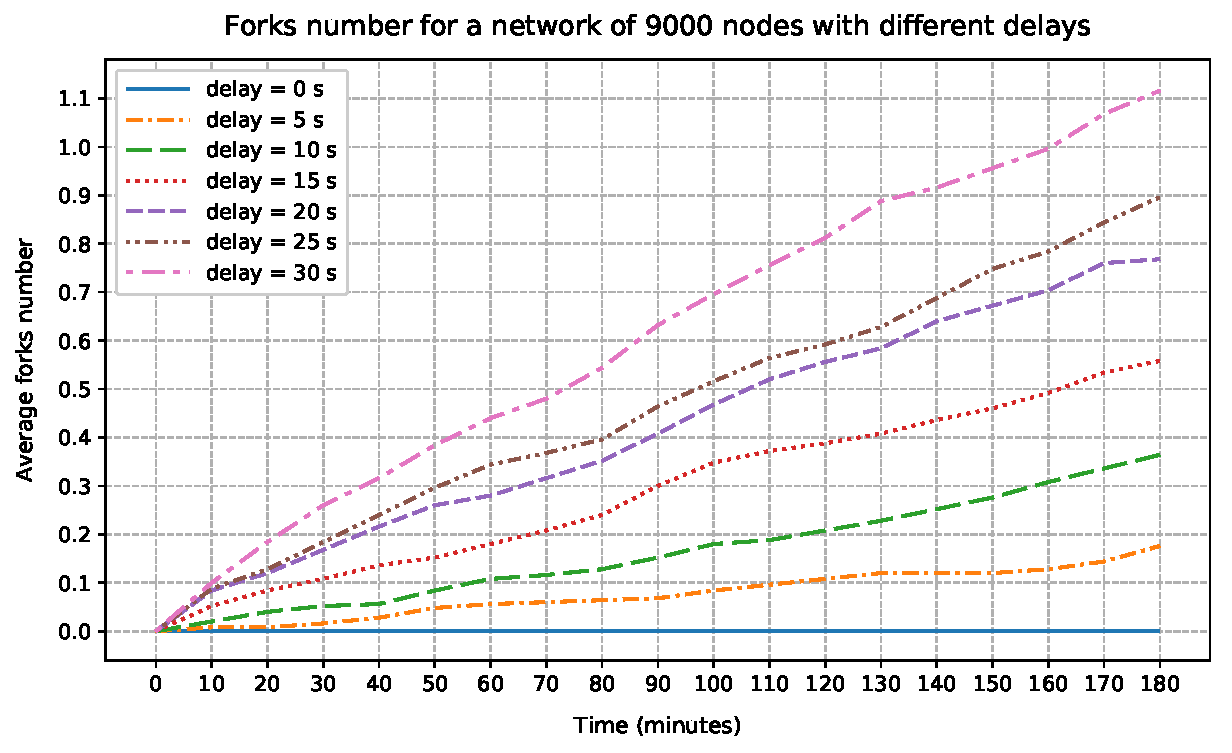
\includegraphics[width=\myplotswitdth \columnwidth]{plots/forks_delay_9000_linechart}
		\vspace*{0.25cm}
		\caption{
			Average forks number for a network of \num{9000} nodes with different delays.
			With short delays, the average number of forks is small.
			With longer delays, Bitcoin generates on average about \num{1} fork every \num{3} hours.
		}
		\vspace*{0.75cm}
	\end{subfigure}
	\begin{subfigure}{\textwidth}
		\centering
		\vspace*{0.25cm}
		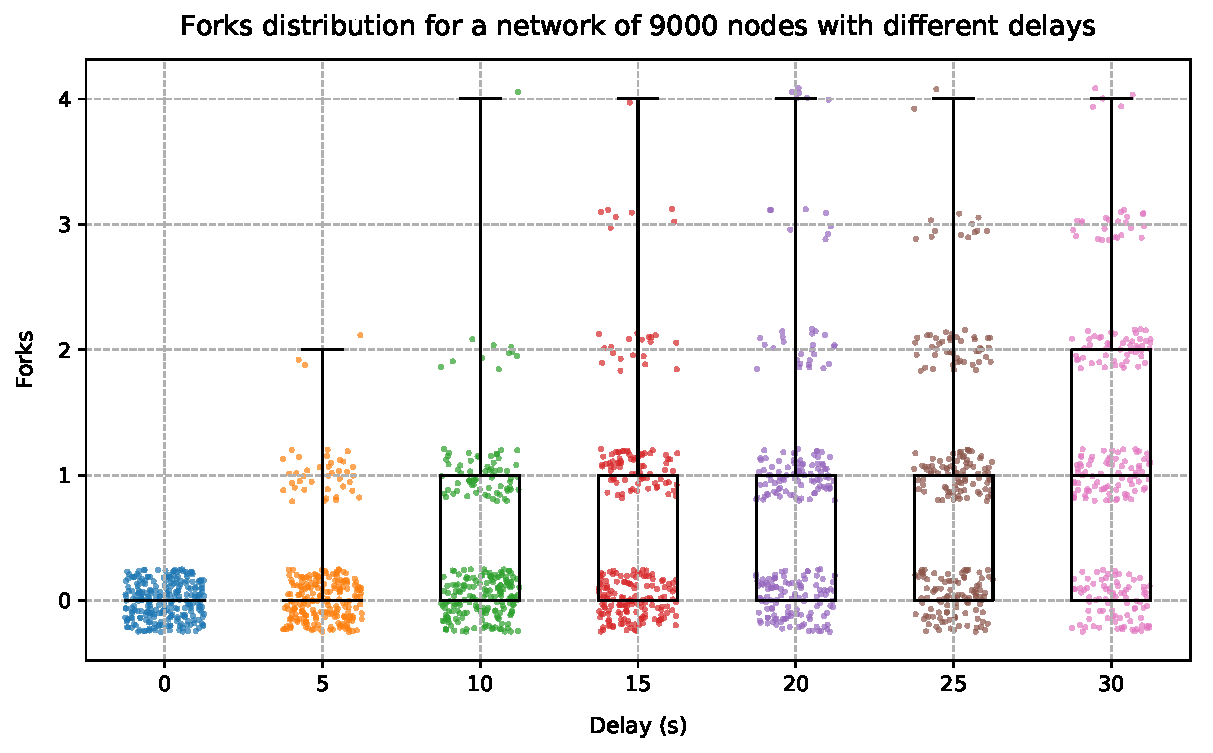
\includegraphics[width=\myplotswitdth \columnwidth]{plots/forks_delay_9000_boxplot}
		\vspace*{0.25cm}
		\caption{
			Distribution of forks for a network of \num{9000} nodes with different delays.
			With zero delay, blocks are immediately distributed to all nodes and no fork is generated.
			As for smaller networks, even a small delay of \num{5} s starts to create some forks, and longer delays produce an higher number of forks.
		}
		\vspace*{0.25cm}
	\end{subfigure}
	\caption[Forks distribution for a network of 9000 nodes with different delays]{
		Forks distribution for a network of \num{9000} nodes with different delays.
	}
	\label{fig:forks-delay-9000}
\end{figure}

\subsection{Balance Attack}

\subsubsection{Delay}
We first fix the size of the network and explore the effect of base Balance attacks with different values of \texttt{balance\_attack\_delay}, then we fix a delay and explore its effect on networks with different sizes.
For all experiments in this section, we fix a base network delay of \SI{50}{\milli\second}.

\medskip
\cref{fig:forks-attack-delay-1000} shows the effect of a Balance attack on a network of \num{1000} nodes.
The growth of forks over time seems to be linear for all tested delays.
Even with a small delay of \SI{10}{\second} on the propagation of \texttt{Block} messages, the network generates on average about \num{0.7} forks in \num{3} hours of simulation;
the number of forks is distributed around \num{1}, but reaches \num{2} or \num{3} in many simulations.
The distribution of the number of forks for longer delays follows a similar behavior, but it is shifted towards higher numbers:
with a delay of \SI{30}{\second}, the network generates up to \num{4} - \num{6} forks, a very high number if compared with the \num{18} expected blocks.

\begin{figure}[ht]
	\begin{subfigure}{\textwidth}
		\centering
		% \vspace*{0.25cm}
		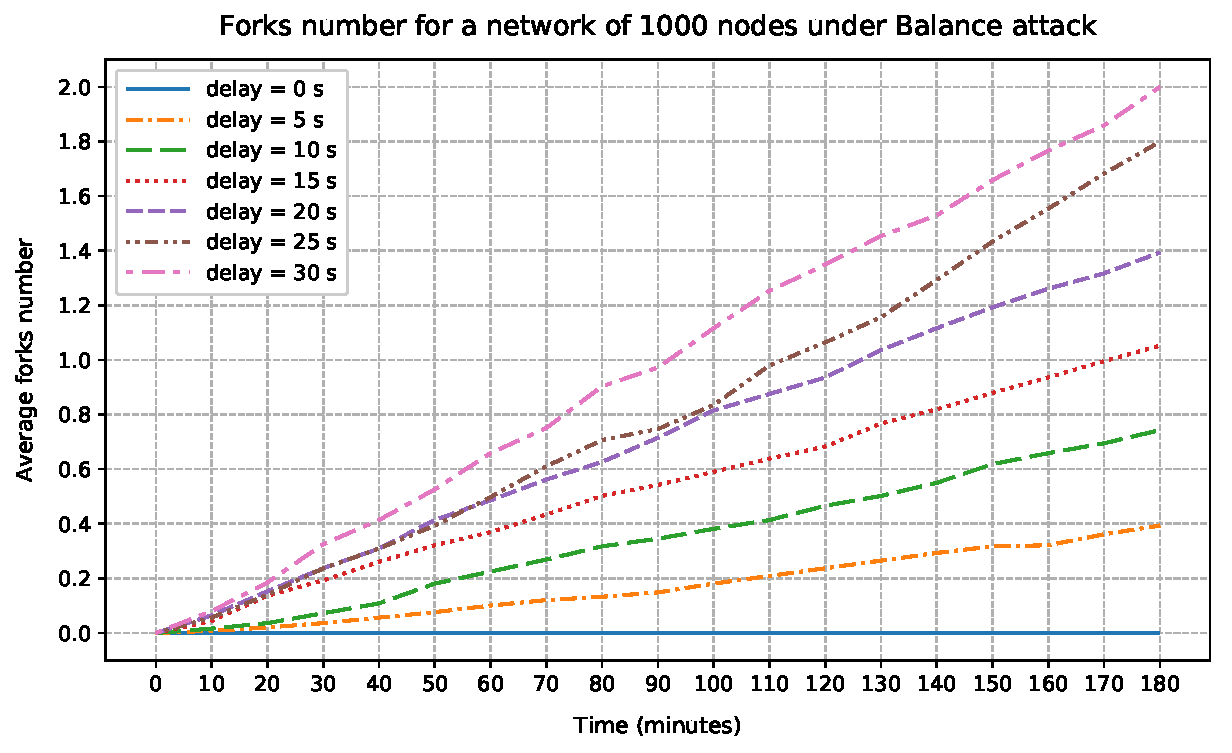
\includegraphics[width=\myplotswitdth \columnwidth]{plots/forks_attack_delay_1000_linechart}
		\vspace*{0.25cm}
		\caption{
			Average forks number for a network of \num{1000} nodes under Balance attack.
			Relatively small delays of \SI{10}{\second} on the propagation of \texttt{Block} messages between nodes belonging to different partitions cause \num{0.7} fork on average at the end of the \num{3} hours simulation.
			With a larger delay of \SI{30}{\second}, the average number of forks raises to \num{2}.
		}
		\vspace*{0.75cm}
	\end{subfigure}
	\begin{subfigure}{\textwidth}
		\centering
		\vspace*{0.25cm}
		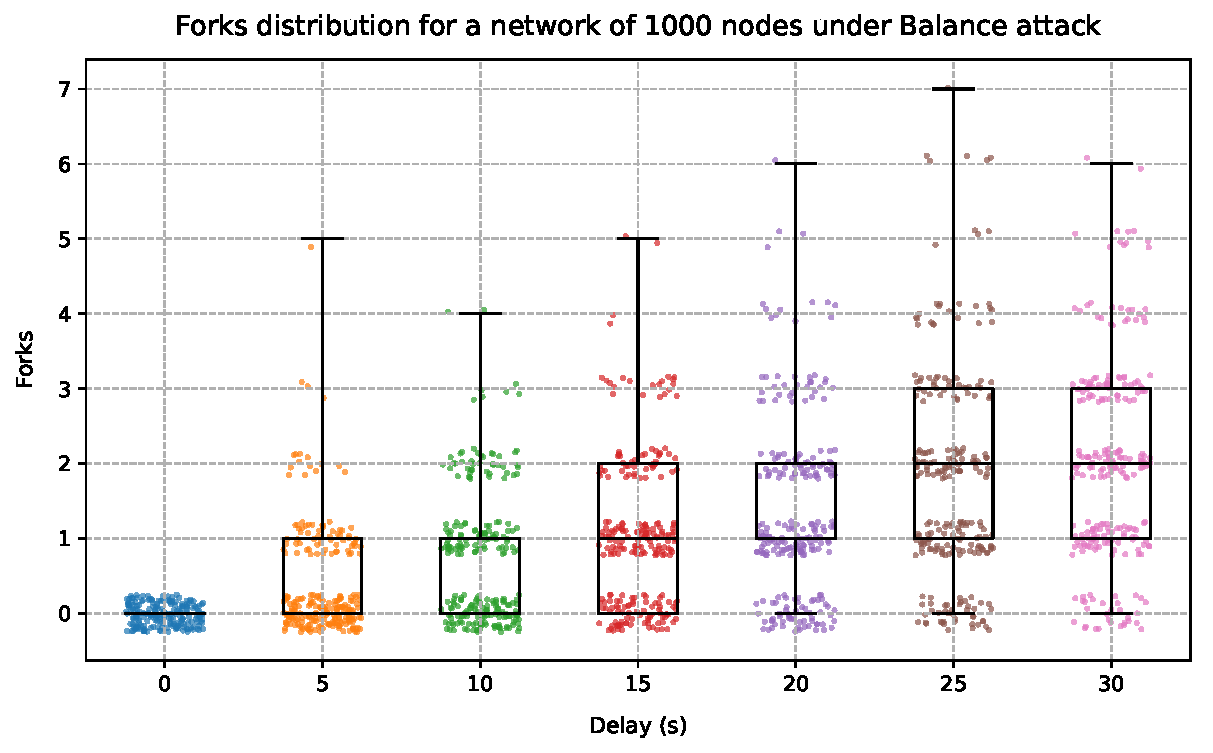
\includegraphics[width=\myplotswitdth \columnwidth]{plots/forks_attack_delay_1000_boxplot}
		\vspace*{0.25cm}
		\caption{
			Distribution of forks for a network of \num{1000} nodes under Balance attack.
			Many simulations with delay of \SI{10}{\second} generate \num{1} fork, while some have reached \num{2} or \num{3} forks.
			The distribution of forks shifts towards higher numbers with larger delays.
			With a delay of \SI{30}{\second}, the network generates up to \num{4} - \num{6} forks.
		}
		\vspace*{0.25cm}
	\end{subfigure}
	\caption[Forks distribution for a network of 1000 nodes under Balance attack]{
		Forks distribution for a network of \num{1000} nodes under Balance attack.
	}
	\label{fig:forks-attack-delay-1000}
\end{figure}

\medskip
\cref{fig:forks-attack-sizes} shows the effect of the Balance attack for a fixed delay of \texttt{Block} messages on network of different sizes.
With both a delay of \num{30} and \SI{60}{\second}, there is no significant difference in the distribution of forks for the different networks.
For all sizes, longer delays cause a higher number of forks on average.

\begin{figure}[ht]
	\begin{subfigure}{\textwidth}
		\centering
		% \vspace*{0.25cm}
		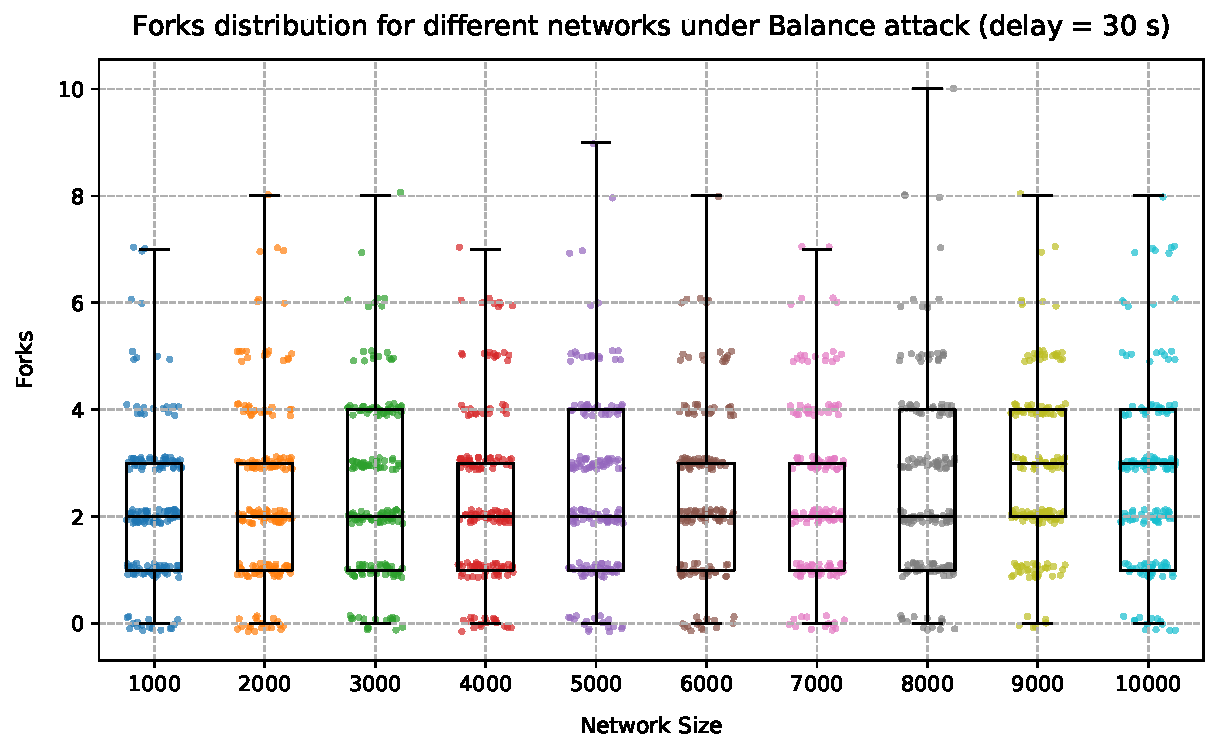
\includegraphics[width=\myplotswitdth \columnwidth]{plots/forks_attack_delay_30_network_sizes_boxplot}
		\vspace*{0.25cm}
		\caption{Forks distribution for different networks under a Balance attack that delays all \texttt{Block} messages by \SI{30}{\second}.}
		\vspace*{0.75cm}
	\end{subfigure}
	\begin{subfigure}{\textwidth}
		\centering
		\vspace*{0.25cm}
		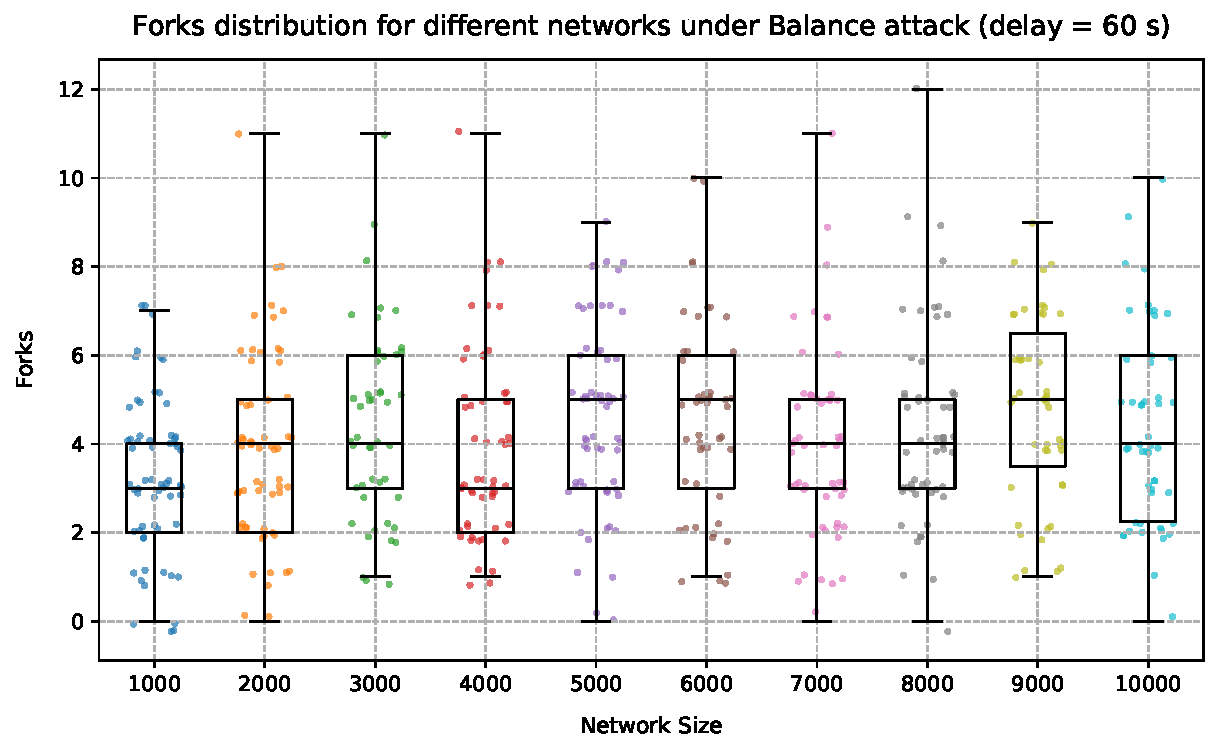
\includegraphics[width=\myplotswitdth \columnwidth]{plots/forks_attack_delay_60_network_sizes_boxplot}
		\vspace*{0.25cm}
		\caption{Distribution of forks for different networks under a Balance attack that delays all \texttt{Block} messages by \SI{60}{\second}.}
		\vspace*{0.25cm}
	\end{subfigure}
	\caption[Forks distribution for different networks under Balance attack]{
		Distribution of forks for different networks under a Balance attack that delays all \texttt{Block} messages by \num{30} or \SI{60}{\second}.
		The size of the network does not seem to influence the effect of the attack for both the tested delays of \num{30} and \SI{60}{\second}.
	}
	\label{fig:forks-attack-sizes}
\end{figure}

\subsubsection{Drop}
We evaluate the effect of dropping \texttt{Block} messages instead of simply delaying them.
\cref{fig:forks-attack-drop} shows the effect of a Balance attack that drops the messages with different probabilities on a network of \num{1000} nodes.
The effect of the attack is almost absent for $\texttt{balance\_attack\_drop} \leq 0.7$.
The attack starts to work for $\texttt{balance\_attack\_drop} = 0.8$ and works very well for $\texttt{balance\_attack\_drop} \in \{0.9, 1\}$.
In other words, the attack works only if most \texttt{Block} messages between nodes in different partitions are dropped.
The gossip mechanism implemented in the Bitcoin protocol to tolerate loss of messages seems to work very well and makes this attack ineffective or impracticable in practice:
if a \texttt{Block} message manages to reach a single node in the other partition, it is immediately gossiped to the entire partition.
Delaying all messages instead of dropping some of them is a much better strategy for the attacker.

\begin{figure}[ht]
	\begin{subfigure}{\textwidth}
		\centering
		% \vspace*{0.25cm}
		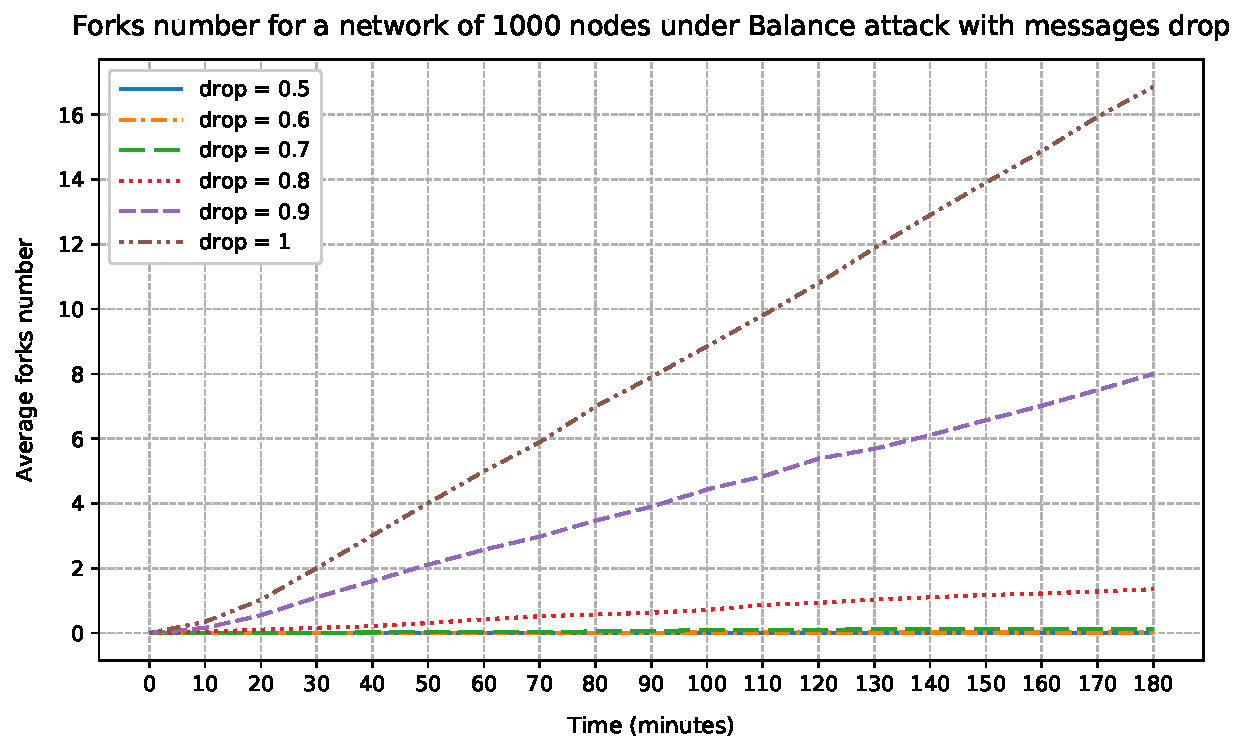
\includegraphics[width=\myplotswitdth \columnwidth]{plots/forks_attack_drop_linechart}
		\vspace*{0.25cm}
		\caption{Average forks number for a network of \num{1000} nodes under a Balance attack with message different drops.}
		\vspace*{0.75cm}
	\end{subfigure}
	\begin{subfigure}{\textwidth}
		\centering
		\vspace*{0.25cm}
		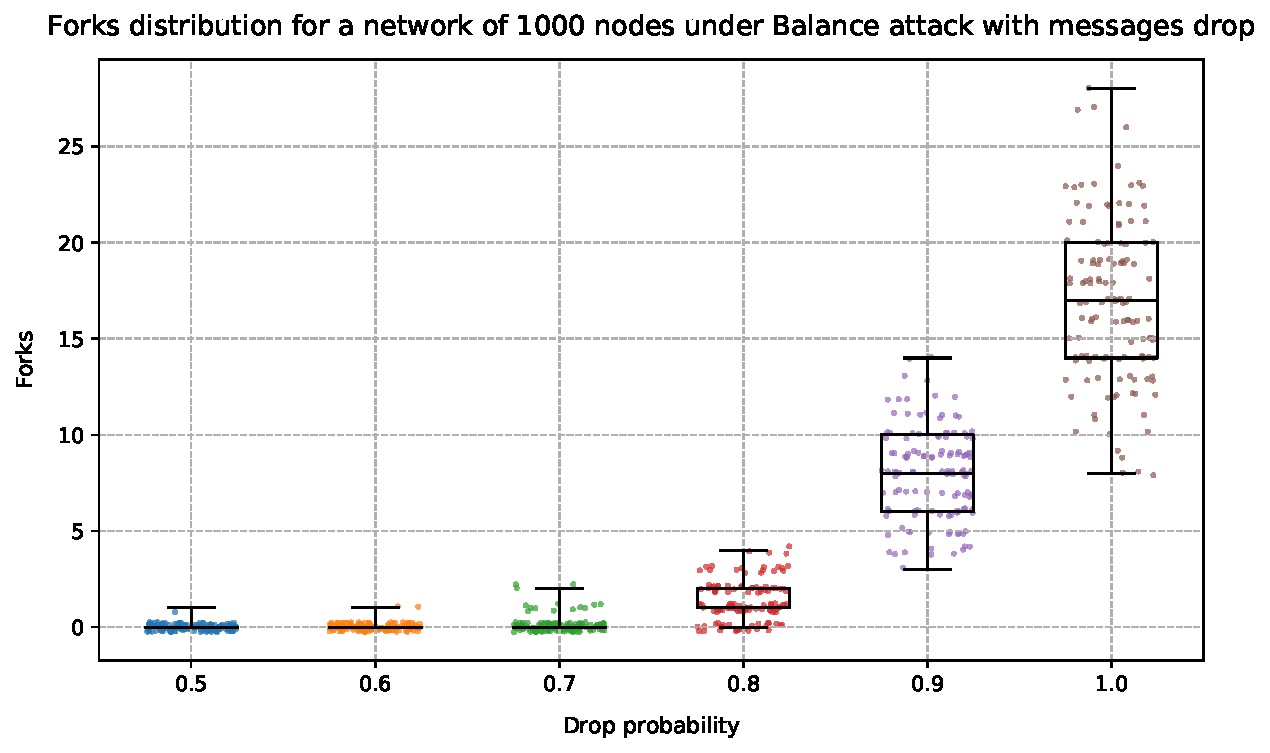
\includegraphics[width=\myplotswitdth \columnwidth]{plots/forks_attack_drop_boxplot}
		\vspace*{0.25cm}
		\caption{Forks distribution for a network of \num{1000} nodes under a Balance attack with message different drops.}
		\vspace*{0.25cm}
	\end{subfigure}
	\caption[Forks distribution for a network of \num{1000} nodes under a Balance attack with different message drops]{
		Forks distribution for a network of \num{1000} nodes under a Balance attack with different message drops.
		The attacks works well only for drop probabilities of \num{0.8} to \num{1}.
	}
	\label{fig:forks-attack-drop}
\end{figure}

% help putting the plots on the correct pages
\clearpage

\subsubsection{Partitions}
We run some experiments to evaluate if the number of partitions created by the Balance attack influence its effectiveness.
\cref{fig:forks-attack-partitions} shows the distribution of forks for a network of \num{1000} nodes during a Balance attack with \texttt{balance\_attack\_delay} of \SI{120}{\second} with different number of partitions.
According to our experiment, there is no significant difference in the effect of the attack for a number of partitions between \num{2} and \num{10}:
the forks are distributed around \num{6}, with most points concentrated around \num{4} and \num{8}.
The results are in line with the previous experiments.

\begin{figure}[t]
	\centering
	\vspace*{0.25cm}
	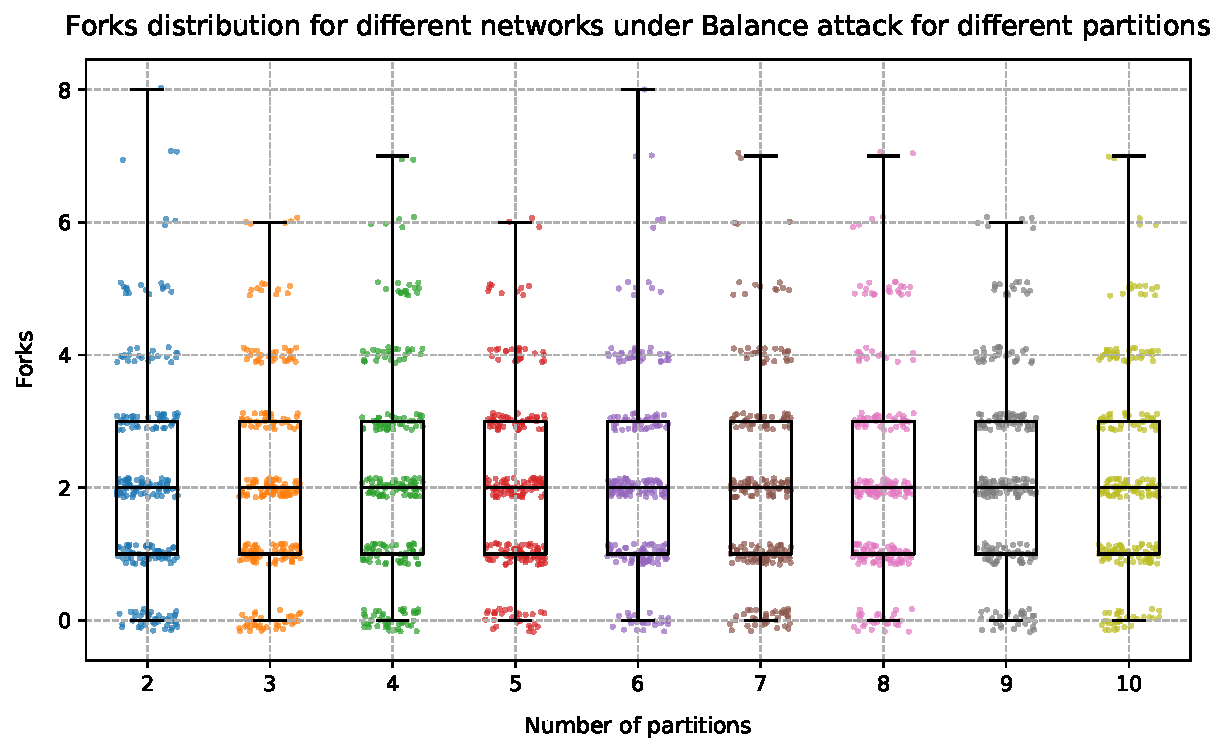
\includegraphics[width=\myplotswitdth \columnwidth]{plots/forks_attack_partitions_boxplot}
	\caption[Forks distribution for a network of 1000 nodes under Balance attack with different numbers of partitions]{
		Forks distribution for a network of 1000 nodes under Balance attack with different numbers of partitions and \texttt{balance\_attack\_delay} of \SI{120}{s}.
		There is not significant difference in the number of forks generated for the different number of partitions.
	}
	\label{fig:forks-attack-partitions}
\end{figure}


\section{Evaluation}
The Balance attack is very effective in creating forks in the Bitcoin's blockchain.
Delaying \texttt{Block} messages between different partitions of about the same size is much more effective than introducing random delays in the entire network.
Dropping random packets between nodes of different partitions is ineffective, thanks to the gossip protocol implemented by Bitcoin to propagate blocks and transactions:
as soon as a single \texttt{Block} message manages to reach the other partition, it is immediately broadcasted to the neighbors, which themselves propagate the information to their peers, until all nodes in the network have received the information.
The attack seems to have the same effect for a different number of partitions (\num{2} to \num{10}), provided they all have about the same size (or better, the same computational power).
